\title{Homework 1 Report}
\author{
        Hooley Cheng \\
                Department of Mathematics\\
        University of Washington\\
        Seattle, WA, 98105, U.S.
           
}
\date{\today}

\documentclass[12pt]{article}
\usepackage{graphicx}
\usepackage{float}
\usepackage{listings}

\usepackage{titlesec}
\begin{document}
\maketitle

\begin{abstract}
This project intends to track the trajectory of a marble swallowed by a dog. Our goal is to de-noise the original ultrasonic data to obtain the path of the object. Alone the way, we used Fourier transformation, Averaging and Gaussian Filter and finally got a clear path of the object.
\end{abstract}

\section{Introduction and Overview}


\paragraph{Problem}
Your dog fluffy swallowed a marble. The vet suspects that it has now worked its way into the intestines.
Using ultrasound, data is obtained concerning the spatial variations in a small area of the intestines where the
marble is suspected to be. Unfortunately, fluffy keeps moving and the internal fluid movement through the
intestines generates highly noisy data.
\paragraph{Method}
We will discuss how we finally found a way by using Fourier Transformation, Averaging and Gaussian to deal with this problem.
\begin{figure}[H]
  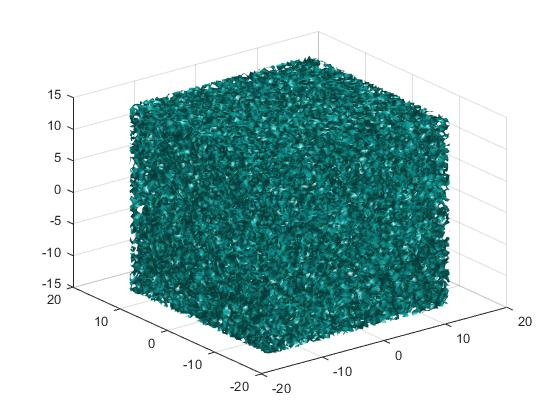
\includegraphics[width=0.7\linewidth]{original_data_1.jpg}
  \caption{One example of original ultrasonic data}
  \label{fig:original_data}
\end{figure}
\section{Theoretical Background}
As described in the problem, the marble is keep moving and internal fluid makes noise. 
So, our first goal is de-noising. Since we have multiple data of same area, the first idea is to average them and, hopefully, noise will be cancelled. However, the object is moving, we cannot use this trick in the time domain. Therefore, we decide to transform all those data into frequency domain. Here is our explanation of why doing so.

\begin{figure}[H]
  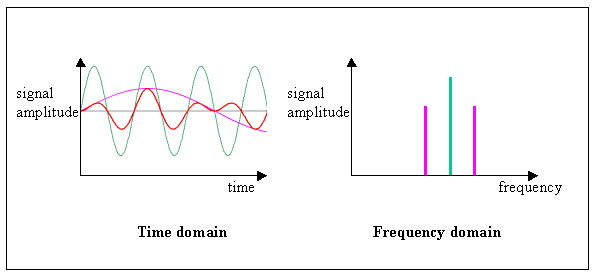
\includegraphics[width=\linewidth]{time_domain_vs_frequency_domain.jpg}
  \caption{some singal on its time domain and its corresponding frequency domain}
  \label{fig:time_frequency}
\end{figure}

An easy to understand reason is that we want to make our object in some way to be static, and that will help us to average noise. And, a certain object regularly reflects same frequency of wave, therefore, if we could transform our original data into frequency domain, the objective frequency we are looking for will be static.\\
Hence, we decide to use Fourier Transformation which precisely does the job. We consider the amplitude $y$ to be the range of a certain function $f(\bf x)$ on time domain where $\bf x$ is a vectorized time realization and which $y = f( {\bf x}) $. Then, 

 \[ F({\bf k}) = \frac{1}{\sqrt{2\pi}} \int_{-\infty}^{\infty} e^{-ik{\bf x}}f({\bf x}) d{\bf x} \]
 could help us transform the function into frequency domain. Notice that, ${\bf k}$ is a vectorized frequency realization.
 
 After these steps, we now can simply average all transformed data and seek for the peek amplitude which should be located around the objective frequency.
 Now, we have our target, ${\bf k}$, and the next work is to minimize all other frequency from our sequence. Here, we decide to use Gaussian Filter which will filter out all values rather than central frequency.\\

Mathematically,
 \[G({\bf k}) = e^{-\tau(\bf k - k_0)^2}\]
 where $\tau$ generally describes the "width of the window" of the filter, and $\bf k_0$ is the central frequency, namely, our target.\\
Also, the inverse Fourier Transformation is:
\[ f({\bf x}) = \frac{1}{\sqrt{2\pi}} \int_{-\infty}^{\infty} e^{-ik{\bf x}}F({\bf k}) d{\bf k} \]
Finally, we found all knowledge required to solve this problem. We then apply the Gaussian Filter with correct $\bf k_0$ we found and use inverse Fourier Transformation, and, hopefully, we eventually found the marble and save the dog.
 
\section{Algorithm Implementation and Development}
As implementation, reality always differs from theory. First we need to Transform all those data into frequency domain and, meanwhile, we sum them up to average(\textit{See Appendix B Listing 2 For Source Code}).\\
	
In order to find the central frequency, we need to visualize the averaged data. However, the expectation of noise is not zero, so we decide to find the mean value (about 56) which should be an approximation of background noise. Here is the visualization after filtering out all noise under value 56:
\begin{figure}[H]
  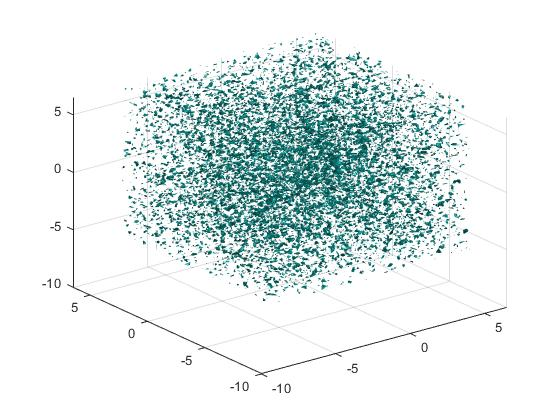
\includegraphics[width=0.7\linewidth]{56.jpg}
  \caption{filtering out values under 56.}
  
  \label{fig:original_data}
\end{figure}
Unfortunately, this image is still noisy. We then decide to find the maximum of the data which should be an approximation of $F(\bf k)$ of the central frequency, (and this value is around 271). Then, we made an assumption that the mid point of these two values should be a efficient boundary that filter out most noise. And, hopefully, we get:
\begin{figure}[H]
  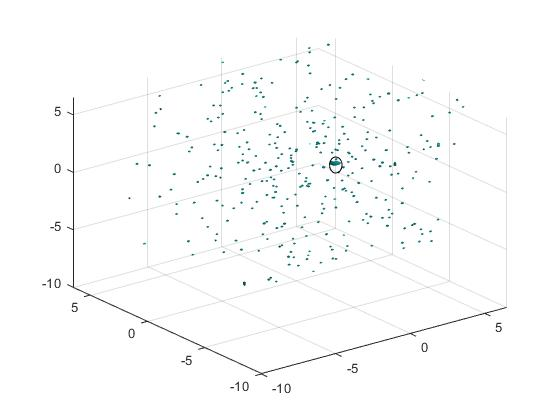
\includegraphics[width=0.7\linewidth]{163.jpg}
  \caption{filtering out values under 163.}
  
  \label{fig:original_data}
\end{figure}
We found a cluster (in the circle above) which differs from any other points. Therefore, we decide to check its $\bf k$ and to see if it is our target. After calculation, we set our ${\bf k} = <1.9895, -0.9426, 0.1047>$, and $\tau = 0.5$ (also tried many times). Finally, after applying Gaussian Filter and Inverse Fourier Transformation, we get a clear trajectory of the marble(\textit{See Appendix B Listing 3 For Source Code}):\\

\begin{figure}[H]
\minipage{0.45\textwidth}
  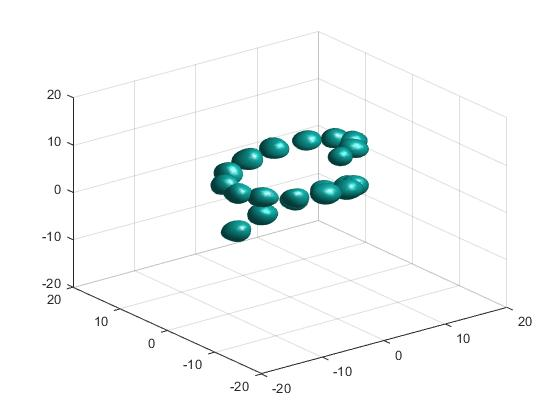
\includegraphics[width=\linewidth]{trajectory.jpg}
  \caption{the isosurface of the path of the marble with iso-value 0.2}\label{fig:awesome_image1}
\endminipage\hfill
\minipage{0.45\textwidth}%
  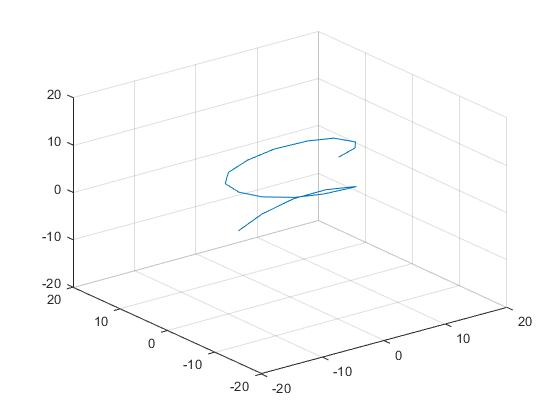
\includegraphics[width=\linewidth]{path.jpg}
  \caption{By tracking the peek value, we also could visualize its path}\label{fig:awesome_image3}
\endminipage
\end{figure}

\section{Computational Results}
the average noise after FFTN is 56.0753\\
the maximum value of average after FFTN is 271.8673\\
the bandwidth $\tau$ of Gaussian Filter is 0.5\\
the central frequency $\bf k$ is $<1.9895, -0.9426, 0.1047>$ \\
the iso-value (or the filter to filter out noise) of the final outcome is 0.2\\
the path data are:
\begin{table}[H]
\begin{tabular}{|l|l|l|l|l|l|l|l|}
\hline
 NO. &X        & Y        & Z        & NO. &X        &Y         &Z  \\ \hline
1  &4.6875   & -4.21875 & 9.84375  &11 &-7.03125 & -3.28125 & 5.15625\\\hline
2  &8.4375   & -2.8125  & 9.84375  &12 &-2.8125  & -4.6875  & 4.21875\\\hline
3  &10.3125  & -0.46875 & 9.375    &13 &1.875    & -4.6875  & 3.28125\\\hline
4  &8.90625  & 2.34375  & 9.375    &14 &6.5625   & -3.75    & 2.34375\\ \hline
5  &6.09375  & 4.21875  & 8.90625  &15 &9.375    & -1.875   & 0.9375\\\hline
6  &1.40625  & 5.15625  & 8.4375   &16 &9.84375  & 0.46875  & -0.46875\\\hline
7  &-3.28125 & 4.6875   & 7.96875  &17 &7.96875  & 2.8125   & -1.40625\\\hline
8  &-7.5     & 3.28125  & 7.5      &18 &4.21875  & 4.6875   & -2.8125\\\hline
9  &-9.84375 & 0.9375   & 7.03125  &19 &-0.9375  & 4.6875   & -4.21875\\\hline
10 &-9.375   & -1.40625 & 6.09375  &20 &-5.15625 & 4.21875  & -6.09375\\\hline  
\end{tabular}
\end{table}
\section{Summary and Conclusions}
Fourier Transform, Averaging and Gaussian Filter together is a very practical tool when analysing noisy signals. As a reminder, the expectation of background noise usually is not zero. Therefore, finding a good boundary when visualizing those data is fairly important when calculating central frequency. Moreover, the imaginary part after FFT needs to be sustained in order to IFFT back to original data.
\section{Appendix A}
Y = fftn(X) returns the multidimensional Fourier transform of an N-D array using a fast Fourier transform algorithm. The N-D transform is equivalent to computing the 1-D transform along each dimension of X. The output Y is the same size as X.\\

X = ifftn(Y) returns the multidimensional discrete inverse Fourier transform of an N-D array using a fast Fourier transform algorithm. The N-D inverse transform is equivalent to computing the 1-D inverse transform along each dimension of Y. The output X is the same size as Y.\\

Y = fftshift(X) rearranges a Fourier transform X by shifting the zero-frequency component to the center of the array.
If X is a vector, then fftshift swaps the left and right halves of X.
If X is a matrix, then fftshift swaps the first quadrant of X with the third, and the second quadrant with the fourth.
If X is a multidimensional array, then fftshift swaps half-spaces of X along each dimension.\\

X = ifftshift(Y) rearranges a zero-frequency-shifted Fourier transform Y back to the original transform output. In other words, ifftshift undoes the result of fftshift.
If Y is a vector, then ifftshift swaps the left and right halves of Y.
If Y is a matrix, then ifftshift swaps the first quadrant of Y with the third, and the second quadrant with the fourth.
If Y is a multidimensional array, then ifftshift swaps half-spaces of Y along each dimension.\\
\section{Appendix B: Matlab Source Code}
\begin{lstlisting}[caption={Starter code}, frame=single]  
clear; close all; clc;
load Testdata
L=15; % spatial domain
n=64; % Fourier modes
x2=linspace(-L,L,n+1); x=x2(1:n); y=x; z=x;
k=(2*pi/(2*L))*[0:(n/2-1) -n/2:-1];
ks=fftshift(k);
[X,Y,Z]=meshgrid(x,y,z);
[Kx,Ky,Kz]=meshgrid(ks,ks,ks);;
\end{lstlisting}

\begin{lstlisting}[caption={N-Dimensional Fast Fourier Transformation and Averaging}, frame=single]
ave=zeros(n,n,n);
for j=1:20
Un(:,:,:)=reshape(Undata(j,:),n,n,n);
ave=ave+fftn(Un);
end
ave = abs(fftshift(ave))/20;
\end{lstlisting}
\begin{lstlisting}[caption={Gaussian Filter and Inverse N-Dimensional Fast Fourier Transformation}, frame=single]
tau=0.5;
tx=1.9895;
ty=-0.9426;
tz=0.1047;
filter = exp(-tau*((Kx - tx).^2+(Ky-ty).^2+(Kz-tz).^2));
filter=ifftshift(filter);
path = zeros(20,3);
for j=1:20
Un(:,:,:)=reshape(Undata(j,:),n,n,n);
fftun=fftn(Un);
res=filter .* fftun;
inv=ifftn(res);
inv=abs(inv);
[mxv,idx]=max(inv(:));
[r,c,p]=ind2sub(size(inv),idx);
path(j,:) = [x(c),y(r),z(p)];
isosurface(X,Y,Z,inv, 0.2)
axis([-20 20 -20 20 -20 20]),grid on, drawnow
end
\end{lstlisting}
\end{document}